\DiaryEntry{Quotient Groups and Homomorphisms}{2023-07-17}{Algebra}

We start with the definition of a homomorphism.

\begin{definition}
Let $(G,\star)$ and $(H,\cdot)$ be two groups. A map $\phi: G \rightarrow H$ such that

\bee
\phi(x \star y) = \phi(x) \cdot \phi(y), \quad \forall x, y \in G
\eee

is called a homomorphism.

\end{definition}

The map $\phi$ need not (and in most cases will not) be one-to-one; in most cases, several elements from $G$ will be mapped to the same element of $H$. The \emph{fibers} are those elements of $G$ projecting to single elements of $H$.

This is illustrated in the following Figure: All elements (represented as dots) in $G$ are mapped to the same element in $H$.

\begin{figure}[H]
\centering
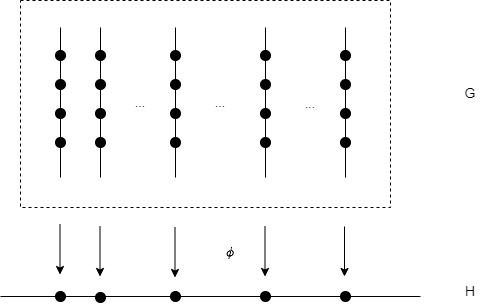
\includegraphics[scale=0.55]{images/2023-07-17-homomorphism.png}
\end{figure}

The classical example is to define $G$ as the numbers in $\mZ$ under the group operation addition $+$. The group $H$ is $\{0, 1\}$ under group operation addition $\mod 2$ (denoted as $\oplus$) and we define the map as $\phi(x) = x \mod 2$. This is a homomorphism, as can be easily checked: eg, we have $(1 + 4) \mod 2 = 5 \mod 2 = 1$ and $(1 \mod 2) \oplus (4 \mod 2) = 1 \oplus 0 = 1$.

 There are two fibers: One is the set of elements in $G$ which are mapped by $\phi$ to $0$ in $H$ and this is the set of even numbers. The other fiber is the set of elements in $G$ which are mapped by $\phi$ to $1$ in $H$ and this is the set of odd numbers.

The group operation in $H$ provides a way to multiply two elements in the image of $\phi$. This suggests a natural multiplication of the \emph{fibers} lying above thw two points , thereby making the set of fibers into a group: If $X-a$ is the fiber above $a$ and $X_b$ is the fiber above $b$, then the product $X_a X_b$ is defined to be fiber $X_{ab}$ above the product $ab$; ie $X_a X_b = X_{ab}$. We can easily show that this defines a group and the group $G$ is partitioned into pieces (the fibers) and these pieces themselves have the structure of a group, called the \emph{quotient group} of $G$.

The \emph{kernel} is the set of elements in $G$ which map to the identity element of $H$; ie the fiber over the identity of $H$.



%%% Local Variables:
%%% mode: latex
%%% TeX-master: "journal"
%%% End:
